
\section{Background}
\label{sec:background}

\begin{figure*}
    \centering
    \begin{subfigure}[t]{0.5\textwidth}
        \centering
        
\includegraphics[height=.7\textwidth]{figs/Depth814.png}
        \caption{Depth (in greyscale)}
        \label{fig:814:depth}
    \end{subfigure}%
    ~ 
    \begin{subfigure}[t]{0.5\textwidth}
        \centering
        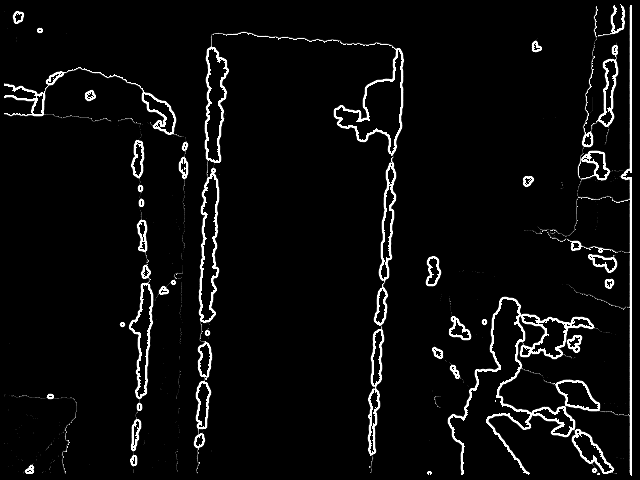
\includegraphics[height=.7\textwidth]{figs/Edged814.png}
        \caption{Edged}
        \label{fig:814:edged}
    \end{subfigure}
    \caption{Edge detection of a doorway and nearby fridge and countertop using the Marr-Hildreth algorithm.}
\end{figure*}

\subsection{Laplacian Edge Detection (LED)}
\label{subsec:laplacian}
Edge detection distinguishes edges between pixels by locating large discontinuities in the data of adjacent pixels. In color images, two different
objects often have very different luminosities, colors, or
patterns; edge detection locates the areas where the pixels
experience a rapid change in those values. While pixels in RGB images
have various characteristics, depth image pixels only have one
piece of data (the depth). Thus, edge detection in depth images
locates objects in an image by finding the areas in which the depth
data rapidly changes, known as jump discontinuities. 

The Marr-Hildreth algorithm is one of the simplest forms of edge detection \cite{marr}. A Gaussian blur convolution is applied to the depth image. The blurred image is subtracted from the original image, resulting
in an "edged" image, such as in Fig.~\ref{fig:814:edged}. Areas with similar values across pixels are
relatively unchanged after the blur.   The difference between the original image and the blurred image is therefore small over that area, resulting in small values at that location in the edged image. In contrast, areas with large
differences in values appear significantly different in the blurred image, and as such have large values at that location in the edged image. When rendered in color, the edged image is dark in continuous areas of the depth image but bright in areas with significant discontinuities. 

It should be noted that the Marr-Hildreth algorithm defines edges, but does not group the pixels within those edges.  Grouping of pixels is left to a simple flood-fill algorithm.

\subsection{Gradient Surface Detection (GSD)}
\label{subsec:gradient}
While the Marr-Hildreth algorithm behaves similarly on both color and depth images, it does not take advantage of the different data provided by a depth image.  The distance values in a depth image give a pixelated 3D view from a single vantage point, providing volumetric information about the scene.  This information is especially valuable when attempting to segment surfaces.

Pulli and Pietik{\"a}inen explore several sophisticated approaches in their discussion of depth image segmentation, including fitting continuous differentiable functions, robust estimators, and least squares approximations to the surfaces \cite{pulli}.  We take a simpler and faster approach, evaluating normal vectors for each pixel, which acts as a local partial derivative, and grouping pixels into surfaces if the normals are sufficiently continuous.  

% Describe any background information that the reader would need to know
% to understand your work. You do not have to explain algorithms or
% ideas that we have seen in class. Rather, use this section to describe
% techniques that you found elsewhere in the course of your research,
% that you have decided to bring to bear on the problem at hand. Don't
% go overboard here --- if what you're doing is quite detailed, it's
% often more helpful to give a sketch of the big ideas of the approaches
% that you will be using. You can then say something like ``the reader
% is referred to X for a more in-depth description of...'', and include
% a citation.\\
% Alternately, you may have designed a novel approach for the problem
% --- your own algorithm or heuristic, say. A description of these would
% also be placed in this section (use subsections to better organize the
% content in this case).

% % Note the \subsection{} command 
% \subsection{Enumerating}
% \label{subsec:enum}

% Create bulleted lists by using the \texttt{itemize} command (see source code):
% \begin{itemize}
%   \item Item 1
%   \item Item 2
%   \item Item 3
% \end{itemize}
% Create numbered lists by using the \texttt{enumerate} command (see source code):
% \begin{enumerate}
%   \item Item 1
%   \item Item 2
%     \begin{enumerate}
%     \item Sub-item 2a
%     \item Sub-item 2b
%     \end{enumerate}
%   \item Item 3
% \end{enumerate}

% \subsection{Formatting Mathematics}
% \label{subsec:math}

% Entire books have been written about typesetting mathematics in
% \LaTeX~, so this guide will barely scratch the surface of what's
% possible. But it contains enough information to get you started, with
% pointers to resources where you can learn more. First, the basics: all
% mathematical content needs to be written in ``math-mode'' --- this is
% done by enclosing the content within \$ symbols. For example, the code
% to produce $6x + 2 = 8$ is \texttt{\$6x + 2 = 8\$}. Note that this is
% only good for inline math; if you would like some stand-alone math on
% a separate line, use \emph{two} \$ symbols. For example,
% \texttt{\$\$6x + 2 = 8\$\$} produces: $$6x+2 = 8$$ Here are various
% other useful mathematical symbols and notations --- see the source
% code to see how to produce them.

% \begin{itemize}
%   \item Sub- and super-scripts: $e^{x}, a_{n}, e^{2x+1}, a_{n+2}, f^{i}_{n+1}$
%   \item Common functions: $\log{x}, \sin{x}$
%   \item Greek symbols: $\epsilon, \phi, \pi, \Pi, \Phi$ % capitalizing the first letter produces the upper case letter
%   \item Summations: $\sum_{i=0}^{i=100} i^{2}$ % looks nicer if you typeset it on its own line using $$
%   \item Products: $\prod_{i=0}^{\infty} 2^{-i}$
%   \item Fractions: $3/2$ % prefer this look for inline math
%     $$\frac{x + 5}{2 \cdot \pi}$$\\ % only looks nice when typeset on its own line
% \end{itemize}

% \noindent Other useful resources:
% \begin{itemize}
% \item Find the \LaTeX~command you're looking for by drawing what you
%   want to produce\footnote{Thanks to Dr. Kate Thompson for pointing me
%     to this resource. Also, this is how you create a footnote. Also,
%     don't overuse them --- prefer citations and use the
%     acknowledgements section when possible. I usually only use
%     footnotes when I want to link to include a pointer to a web
%     site.}:\url{http://detexify.kirelabs.org/classify.html}
% \item Ask others: \url{http://tex.stackexchange.com/}
% \item Every \LaTeX~symbol ever:\\ \url{http://tinyurl.com/6s85po}

% \end{itemize}


